\documentclass[../interim.tex]{subfiles}


\begin{document}

\chapter{Project Plan}

In order to provide a plan of the work to be completed, this chapter firstly describes what has been achieved so far, provides possible solutions to some of the key problems which need to be solved and outlines possible methods for evaluating the performance of a completed system.

\section{Completed Work}

Many VideoQA datasets were outlined in the related work discussion in Chapter~\ref{chapter:related}. However, these pre-existing datasets do not contain the semantic information required to extract symbolic properties from objects in each frame. Most of these datasets provide nothing more than a sequence of images, a question and an answer. While this is sufficient to train an end-to-end neural network, since it learns implicit features, it does not allow us to train a network which can extract explicit object properties, which are required for logical reasoning. Although it would be possible to extract some information using a network pre-trained on ImageNet~\cite{imagenet}, for example, we would only be able to extract bounding boxes and classes for each object, whereas we would prefer to extract richer details such as colour, rotation or size. Furthermore, we cannot guarantee that every object in a scene is be part of the ImageNet dataset, and so we may miss objects entirely.

For this reason we have decided to generate a dataset which provides the information needed for logical reasoning, as a starting point for building our model. The dataset emulates a simple retro game environment. Since the focus of this project is to investigate logical reasoning and the learning of symbolic rules we do not attempt to make the job of the neural network difficult by creating very complex scenes. An example frame from the current version of the dataset is shown in Figure~\ref{fig:dataset-frame}. The key elements of the dataset are the following:
\begin{itemize}
  \item \textbf{Octopus}. The `main' character in the frames - the octopus is the only character which moves and its characteristics change as it comes into contact with other objects.

  \item \textbf{Fish}. The fish are always silver, but can have any rotation. When the octopus comes close to the fish, the fish disappears (is eaten).

  \item \textbf{Plastic Bag}. Similarly to the fish, the plastic bags are always white but can have any rotation. Each bag is harmful to the octopus, so both objects disappear when in close contact.

  \item \textbf{Rock}. Rocks can have four colours: brown, blue, purple and green, but always face upright. While an octopus is near a rock the octopus' colour will match that of the rock (it will be camouflaged).
\end{itemize}

The idea behind the dataset is to make these object property changes challenging for ILASP to learn. This is, however, a very early version of the dataset and we may well be required to add more objects with more complex semantics in later stages of the project. We do not attempt to make it difficult for a network to learn to extract properties from the frame, indeed each frame is very simple with a flat background and no variation of object shapes. Each image is also quite small at only 128x128 pixels, this will allow faster network training.

Each object in each frame is labelled with the following information:
\begin{itemize}
  \item \textbf{Class}. The object type, as described above.

  \item \textbf{Bounding Box}. We provide the upper left and lower right coordinates of the box around the object.

  \item \textbf{Colour}. The current colour of the object.

  \item \textbf{Rotation}. The direction the object is currently facing in. This is given as an integer between 0 and 3.
\end{itemize}

\begin{figure}
  \centering
  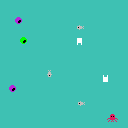
\includegraphics[width=0.5\textwidth]{example-frame.png}
  \caption{An example frame from the initial version of the dataset.}
  \label{fig:dataset-frame}
\end{figure}


\section{Implementation Plan}

\section{Evaluation Plan}


\end{document}
